%! Author = wolfram_e_laube
%! Date = 06.05.24

\item[(c)]
\subsection{Task (c): Qualitative Spectrum Drawing of $x(t)$ up to 20 kHz}

\subsubsection{Problem Statement}
Qualitatively draw the spectrum of the analog signal $x(t)$ up to 20 kHz, considering the effect of zero-order hold (ZOH) reconstruction. Delta pulses should be drawn with an arrow, where the height of the arrow indicates the weight of the delta-pulse.

\subsubsection{Background and Analysis}
\begin{enumerate}
    \item \textbf{Zero-Order Hold (ZOH) Characteristics:}
    The zero-order hold DAC holds each discrete signal value constant over the sample interval, effectively creating a step function between samples. The impulse response of this operation is a rectangular pulse, whose Fourier transform is a sinc function, resulting in a sinc-shaped spectrum that modifies the frequency components of the original signal.

    \item \textbf{Spectral Components:}
    \begin{itemize}
        \item \textbf{Base Frequency:} The original discrete-time signal $x[n]$ has a fundamental frequency of 1000 Hz, resulting in a corresponding delta pulse in the spectrum.
        \item \textbf{Power Calculation:} The power of a sinewave with amplitude $A$ is given by $P = \frac{A^2}{2}$. For $x[n]$, $A = \sqrt{2}$, so $P = 1$ watt, which will be represented by the height of the delta pulse at 1000 Hz.
    \end{itemize}

    \item \textbf{Sinc Function Influence:}
    The frequency response of the ZOH is given by a sinc function, which affects the amplitude of the spectral components. This influence results in a primary lobe around the baseband frequency and side lobes that attenuate in amplitude as they move away from the center frequency.

    \item \textbf{Normalized Sinc:}
    MATLAB and other DSP tools often use a normalized sinc function, which means the function has a maximum of 1 at zero frequency and its first null at the sampling frequency $f_s = 8000$ Hz, serving as a guideline for the drawing.
\end{enumerate}

\subsubsection{Steps for Drawing the Spectrum}
\begin{itemize}
    \item \textbf{Delta Pulse at 1000 Hz:} Mark a delta pulse at 1000 Hz with a height representing the power level of 1 watt.
    \item \textbf{Overlay Sinc Function:} Overlay a sinc function shape across the spectrum. The main lobe should center around 1000 Hz, and side lobes should decrease in amplitude as they extend outwards.
    \item \textbf{Consider Sinc Attenuation:} Show how the sinc function modifies the spectrum, particularly how it attenuates frequencies around 8000 Hz and 16000 Hz just before reaching the nulls.
\end{itemize}

\subsubsection{Conclusion}
The spectrum of $x(t)$ will exhibit characteristics dominated by the sinc function due to the ZOH effect, with a notable delta pulse at the fundamental frequency of 1000 Hz. The qualitative drawing will reflect the sinc function's impact, emphasizing the primary and side lobes up to 20 kHz.

\begin{figure}[h]
    \centering
    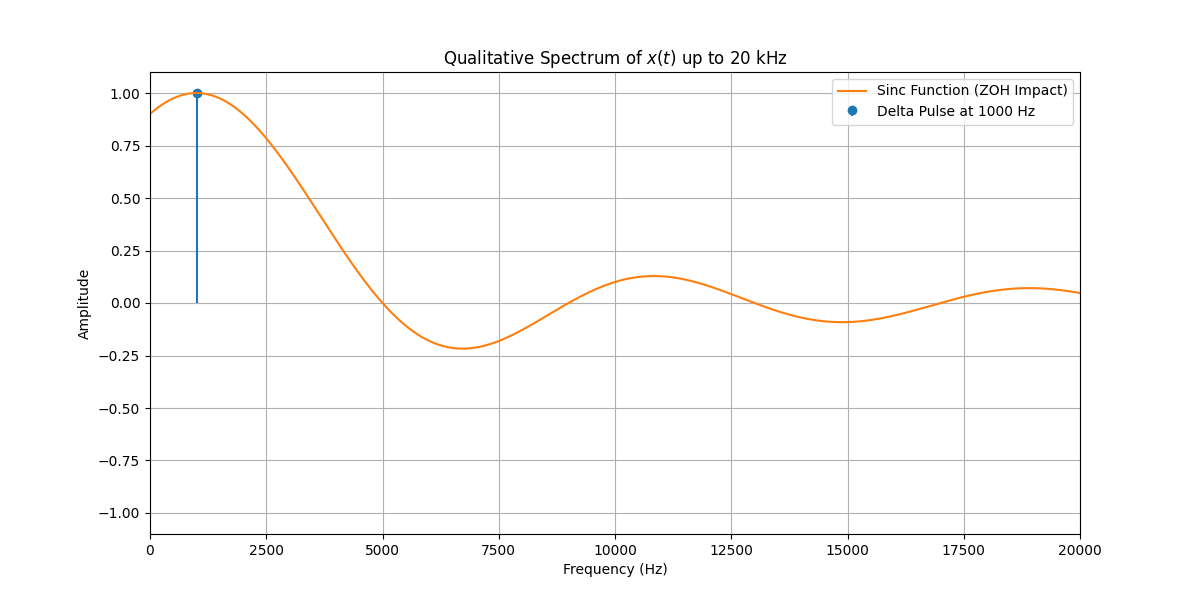
\includegraphics[width=0.49\textwidth]{fig/ex3_c_plot}
    \caption{Qualitative Spectrum of \(x(t)\)}
    \label{fig:ex3_c_plot}
\end{figure}
